\section{Proposed architecture}\label{sec:architecture}
To our knowledge, the only few studies that applied DNN-HMM technique to text-independent SI tasks used deep feed-forward neural networks \cite{si:dnnhmm}, which are hardly able to capture temporal relationships between feature frames due to their sequential structure unlike, for example, Recurrent Neural Networks (RNNs).

On the other hand, as multiple studies in the SI field suggested, the use of 1D/2D Convolutional Neural Networks (CNNs) in combination with log-scaled spectrum/Mel spectrum features can greatly improve the performance of a text-independent SI system, due to the high-level feature extraction power of this type of network \cite{si:lstm}.

This simple observation led us to believe that the combination of the features extracted by both these typologies of networks could lead to even better identification performances, especially if combined to the acoustic modeling power of HMMs.

Thus, the proposed architecture is non-sequential, and combines both convolutional and recurrent layers, trying to combine both kind of features to achieve better performance.

Before describing the mentioned architecture, an overview of the most important network designs that make up its layers will be given.

\subsection{Recurrent Neural Networks (RNN)}
A recurrent neural network (RNN) is a neural network that is specialized in processing a temporal sequence of data $x_1, \cdots,x_T$.

The term "recurrent" in their name refers to the execution of the same operations on each element $x_t$ of the sequence performed by this type of network, applying the same matrix of weights $V$.

This causes each output $o_t$ to depend on the previous ones, and for the network to maintain a hidden state $h_t$ directly dependent on the previous one $h_{t-1}$.

The image \vref{fig:recurrent_neural_network_unfold} shows an RNN unfolding over time (on the sequence) in a complete network.

\begin{figure}
	\includegraphics[width=0.5\textwidth]{images/recurrent_neural_network_unfold}
	\caption{Unrolling of a basic recurrent neural network, compressed on the left and unfolded on the right, source~\cite{wiki:rnn}.}
	\label{fig:recurrent_neural_network_unfold}
\end{figure}

We are going to analyze each element of the architecture of an RNN, explaining step by step how the information is processed within this type of network:
\begin{description}
	\item[input]: $x_t$ represents the input of the network at instant $t$;
	\item[hidden state]: $h_t$ represents the hidden state at time $t$, which acts as the "memory" of the network, being computed based on $x_t$ and the previous state $h_{t-1}$ by applying weight matrices, and an activation function $f$ (any nonlinear transformation such as $\tanh$, ReLU, $\dots$) and adding a bias vector $c$:
	$$
	h_{t}=f\left(U \cdot x_{t}+V \cdot h_{t-1}+c\right)
	$$
	\item[weights]: the connections between neurons of input-to-hidden type ($x_t$ to $h_t$) are parameterized by a matrix of weights $U$, while those of hidden-to-hidden type ($h_{t-1}$ to $h_t$) and hidden-to-output type ($h_t$ to $o_t$) are respectively parameterized by two weight matrices $V$ and $W$;
	\item[output]: $o_t$ represents the output of the network, which is also often subject to a nonlinear activation function $g$, especially when the network contains other layers.
	$$
	o_{t}=g\left(b_{t}+W \cdot h_{t}\right)
	$$ 
	where $b_{t}$ is the bias vector at time $t$
\end{description}


\subsection{Long-Short-Term-Memory (LSTM)}

An LSTM is a special type of RNN. RNNs use recurrent units to learn temporal features from sequence data, as LSTMs do. However, what happens inside the recurrent unit is very different between the two, as shown in image \vref{fig:lstm}.


\begin{figure}
	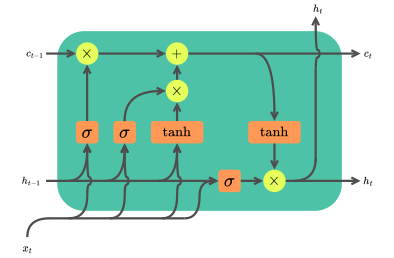
\includegraphics[width=0.5\textwidth]{images/lstm}
	\caption{LSTM unit, source \cite{wiki:lstm}.}
	\label{fig:lstm}
\end{figure}

Assuming we know the basic operation of RNNs, we are going to describe the operation of an LSTM layer at time $t$, to which comes the time sequence $x_1, x_2, \cdots, x_T$:

\begin{description}
	\item[Hidden state and input]: the hidden state of a previous time step $h_{t-1}$ and the input of the current time step $x_t$ are combined before running copies through various operational gates using concatenation between vectors.
	$$
	\left[h_{t-1} \mid x_{t}\right]
	$$
	\item[Cell state:] $c_{t-1}$ is a recurrent input representing the long-term memory of the network. In fact, it will be modified only slightly by the current time step with a sequence of linear additions and Hadamard products (component-wise), resulting in the next cell state $c_t$.
	\item[Forget gate:] this gate controls what saved information should be forgotten, and consists of a simple sigmoid neural network layer that multiplies the previous result with a weight matrix $W_f$, adds a bias vector $b_f$ and gives the result as input to a sigmoid activation function. As the sigmoid function varies between 0 and 1, it determines which cell state values should be discarded (multiplied by 0), remembered (multiplied by 1) or partially remembered (multiplied by a value between 0 and 1).
	$$
	f_{t}=\sigma\left(W_{f} \cdot\left[h_{t-1} \mid x_{t}\right]+b_{f}\right)
	$$
	\item[Input gate:] consists of a sigmoid neural layer, which multiplies [$h_{t-1} | x_t$] with a weight matrix $W_i$, adds a bias $b_i$ and gives the result as input to a sigmoid function. Outputs between 0 and 1 identify the important elements of [$h_{t-1} | x_t$] that are to be added to the cell state $c_{t-1}$.
	\item[Proposed update cell state]: consists of a $\tanh$ neural layer, which multiplies [$h_{t-1} | x_t$] with a weight a matrix $W_c$, adds a bias vector $b_c$ and gives the result as input to the activation function $\tanh$. The output $\tilde{c}_t$ determines the candidate values for storage within the cell state.
	$$
	\tilde{c}_{t}=\tanh \left(W_{c} \cdot\left[h_{t-1} \mid x_{t}\right]+b_{c}\right)
	$$
	\item[Update cell state:] the previous cell state $c_{t-1}$ is multiplied by the result of forget gate $f_t$ to remove irrelevant information, and the result is added component by component to the vector of candidate values $\tilde{c}_{t}$, weighted by the output of input gate $i_t$, to finally obtain the next cell state $c_t$.
	$$
	c_{t}=f_{t} \odot c_{t-1}+i_{t} \odot \tilde{c}_{t}
	$$
	\item[Output gate:] consists of a simple sigmoid neural layer that, again, multiplies [$h_{t-1} | x_t$] with a weight matrix $W_o$, adds a bias vector $b_o$ and gives the result in ingress to a sigmoid activation function.
	$$
	o_{t}=\sigma\left(W_{o} \cdot\left[h_{t-1} \mid x_{t}\right]+b_{o}\right)
	$$
	\item[Update hidden state:] the last step is to update the hidden-state $h_{t-1}$.  The current cell state $c_t$ is passed through the activation function $\tanh$ and multiplied component by component with the output gate result.
	$$
	o_{t}=\tanh \left(c_{t}\right) \odot o_{t}
	$$
\end{description}
Finally, the current cell state $c_t$ and hidden state $h_t$ return as input to the recurrent unit, and the process repeats until the sequence ends.

\subsection{Convolutional Neural Network (CNN)}
Convolutional neural network (CNN) is a class of artificial neural networks that has become dominant in various computer vision and signal processing tasks and is attracting interest across a variety of domains.
CNNs are capable to automatically and adaptively learn hierarchies of high-level features through layers of small weight filters representing the features.
Usually, CNN architectures are composed of multiple building blocks, such as convolution layers, batch normalization and pooling layers.


\paragraph{Convolutional Layer} 
A convolutional layer $l_m$ receives as input a signal $\boldsymbol{x}^{(m-1)}$ with $K_{m}$ channels (either raw input or the output of $(m-1)$-th layer) and computes as output a new signal $\mathbf{x}^{(m)}$ composed of $O_{m}$ channels. The output at each channel is known as a \textbf{feature map}, and is computed as \cite{cnnbook}:

$$
\boldsymbol{x}_{o}^{(m)}=g_{m}\left(\sum_{k} \boldsymbol{w}_{o,k}^{(m)}* \boldsymbol{x}_{k}^{(m-1)}+b_{o}^{(m)}\right)
$$
where $*$ denotes the 1D convolution operation:

$$
\boldsymbol{w}_{o, k} * \boldsymbol{x}_{k}[t] = \sum_{p} \boldsymbol{x}_{k}[t - p] \cdot  \boldsymbol{w}_{o, k}[p] \text{, }
$$
where $\boldsymbol{W}_{o,k}^{(m)} \in R^{P_{m}}$ is vector called \textbf{convolutional kernel}, $b_{o}^{(m)} \in \mathbb{R}$ is a bias vector and $g_m$ is the activation function applied to the final result. The convolutional kernel $\boldsymbol{w}_{o, k}^{(m)}$ act as the trainable parameters of a filter that the layer can use to detect or enhance some feature in the incoming signal frames. The weights and the consequent feature detected/enhanced by the filter are learned during the training process just like the weight matrices of fully-connected neural networks or RNN.

\paragraph{Batch Normalization Layer} 
Batch normalization is a technique that aims to accelerate the training of deep neural networks by reducing the shift of internal covariates. 
This is done through a normalization operation that fixes the means and variances of layer inputs at the batch level. This operation also has a number of extremely beneficial "side" effects:
\begin{itemize}
	\item strong reduction in the dependence of gradients on parameter scaling or their initial values, which allows much higher learning rates to be used without the risk of divergence or gradient exploding;
	\item regularization of the activation values of model units, which reduces the need for dropout or other hard-regularization techniques.
\end{itemize}
Batch normalization is applied as follows to a batch $\mathcal{B}$ with $m$ instances \cite{batchnormalization}:

\begin{enumerate}[label=(\roman*), font=\itshape]
	
	\item computes the mean and variance of the batch $\mathcal{B}$:
	
	$$
	\begin{gathered}
		\mu_{\mathcal{B}}=\frac{1}{m} \sum_{i=1}^{m} x_{i} \\
		\sigma_{\mathcal{B}}^{2}=\frac{1}{m} \sum_{i=1}^{m}\left(x_{i}-\mu_{\mathcal{B}}\right)^{2} \\
	\end{gathered}
	$$
	
	\item computes the normalized instance $\hat{x}_{i}$ for each $i \in \{1, 2, ..., m\}$:
	
	$$
	\begin{gathered}
		\hat{x}_{i} = \frac{x_{i} - \mu_{\mathcal{B}}}{\sqrt{\sigma_{\mathcal{B}}^{2} + \epsilon}} \text{, }
	\end{gathered}
	$$
	where $\epsilon$ is a very small value (e.g. machine epsilon) added to prevent division by zero.
	
	\item computes the layer output for the instance $\hat{x}_i$:
	
	$$
	\begin{gathered}
		y_{i} = \gamma \, \hat{x}_{i} + \beta = \operatorname{BN}_{\gamma, \beta}\left(x_{i}\right) \text{, }
	\end{gathered} 
	$$
	where $\gamma$ and $\beta$ are learnable parameters tuned during back-propagation.
\end{enumerate}


\paragraph{Pooling Layer}
The pooling layers of a CNN implement a dimensionality reduction transformation designed to lower the number of trainable parameters for subsequent layers, allowing them to focus on larger areas of the input patterns while retaining most of the information they contain.

Given an input signal $\boldsymbol{x}^{(m-1)}$ with $K_m$, a 1D pooling layer with pool size $P_{m} \in \mathbb{N}$ and strides $\alpha_{m} \in \mathbb{N}$ is a channel-wise operation like the following \cite{cnnbook}:

$$
\boldsymbol{x}_{o}^{(m)}[t] = \kappa \cdot \left( \sum_{p} \left(\boldsymbol{x}_{o}^{(m-1)} \left[\alpha_{m} \cdot t + p \right] \right)^{\rho}\right)^{1 / \rho}
$$
where $\kappa, \rho \in \mathbb{N}$ are fixed parameters depending on the type of pooling we are applying to the data.

It's worth noting that the use of $P_{m}=\alpha_{m}$ corresponds to dividing each channel of the input signal into non-overlapping $P_{m}$ patches (regions) and replacing the values in each region with a single value calculated on the basis of $\rho$ and $\kappa$.

In max pooling layers $(\rho = \infty, \kappa = 1)$, the output of the above formula value is the maximum of the values found in the patch:

$$
\begin{gathered}
	\lim_{\rho \to \infty} \left(\sum_{p} \left(x^{(m-1)}_o\left[\alpha_{m} \cdot t + p\right]\right)^\rho \right)^{1/\rho} = \\
	\max \left\{x^{(m-1)}_o\left[\alpha_{m} \cdot t + p\right] : p \in \{1, 2, ..., P_m\}\right\} \\
\end{gathered}
$$
In average pooling layers on the other hand, which were also used in this study, $(\rho = 1, \kappa = 1/P_m)$, the result is the average of the values:

$$
\boldsymbol{x}_{o}^{(m)}[t] = \frac{1}{P_m} \cdot \sum_{p} \boldsymbol{x}_{o}^{(m-1)} \left[\alpha_{m} \cdot t + p \right]
$$
	


\subsection{RecConvSiameseNet}\label{subsec:recconvsnet}
Let us now go into a detailed description of the neural network architecture used in the performed experiments.

\paragraph{Branches}
The proposed architecture (Figure \vref{fig:full_architecture}), named RecConvSiameseNet, involves two information processing branches:
\begin{itemize}
	\item one characterized by LSTM recurrent layers (Rec);
	\item the other featuring several 1D convolutional blocks (Conv), each containing a set of increasing 1D convolutional filters, a batch normalization layer and a 1D average pooling layer, followed by a final dense layer which flattens the feature maps extracted by the convolutional blocks.
\end{itemize}
These two branches receive as input two different types of audio features, extracted upstream during preprocessing, which are respectively:
\begin{itemize}
	\item the more refined $(243 \times 39)$ frames containing MFCCs \& deltas;
	\item the coarsest log-scaled Mel spectrum features contained in $(243 \times 128)$ frames.
\end{itemize}

The "Siamese" part in the name refers to the non-sequential nature of the network, which is typical of Siamese networks \cite{siamesenn}, although the proposed architecture does not have the usual characteristics of Siamese networks, the two branches being completely different from each other.

The basic idea, as mentioned earlier, is to combine the features that these two types of layers are capable to extract, in particular:

\begin{itemize}
	\item LSTM branch being fed with MFCCs \& deltas one $(1 \times 39)$ frame at time, and processing them in the same way, it is able to extract temporal-wise features from the cepstrum, capturing short-term and long-term relationship between frames;
	
	\item convolutional branch being fed with the $(243 \times 128)$ log-scaled Mel spectrum features in their entirety, it is capable of excerpting high-level features that span the entire audio.
\end{itemize}

\begin{figure}
	\centering
	\includegraphics[width=0.5\textwidth]{images/full_architecture}
	\caption{DNN-HMM Architecture}
	\label{fig:full_architecture}
\end{figure}
Further details on architecture and implementation of the two branches will be provided in the sections \vref{subsec:cnnautoencoder} and \vref{subsec:recautoencoder}, where the autoencoder models used during the pre-training phase will be described, as the two RecConvSiameseNet branches were extracted from them prior to the training.

\paragraph{Network tail}
As shown in the Figure \vref{fig:full_architecture}, after the feature extraction process done by the the two branches is completed, the LSTM branch result vector $u_t$ is, at each timestep $t$, concatenated with the flattened feature maps extracted by the convolutional branch $v$ (through repeat vector and concatenation layers), resulting in a new feature vector $w_t = [u_t | v]$. This feature vector is fed into a single network tail, composing of two time-distributed dense layers.

The first one has $\nspeakers \cdot \statesspeakers = 5040$ neuron units, and uses units Leaky ReLU activation function \cite{leakyrelu}, with $\alpha = 0.1$:

$$
\leakyrelu(x) := 
\begin{cases}
	x, & x \geq 0 \\
	\alpha x, & x < 0
\end{cases}
$$
The second one has $\nspeakers \cdot \statesspeakers = 5040$ neuron units too, but since it's the final output layer, it aims to predict the posterior probabilities $P(s_t = k \, | \, o_t)$ of each HMM state $k$ given the current frame $o_t$, and thus uses the softmax activation function (like the one we described in previous section \vref{subsec:dnn}).

Denoting with $W_0, b_0$ and $W_1, b_1$ the weights and biases of the first and second tail dense layers, respectively, the network output on each state can be expressed as:

$$P(s_t = k \, | \, o_t) = \sigma(a_t^T \cdot W_1 + b_1)_k \text{, where: }$$

$$a_t = \leakyrelu(w^T \cdot W_0 + b_0)$$
Details about RecConvSiameseNet training procedure and will be described in section \vref{subsec:recconvsnet_train}, while the architecture of the tail can be seen in Table \vref{tab:tail_recconvsnet}.

\begin{footnotesize}
	\begin{table}
		\centering
		\caption{Parameters of RecConvSiameseNet tail}
		\label{tab:tail_recconvsnet}
		\begin{tabularx}{0.5\textwidth}{XXr}%lMr
			\toprule
			\textbf{Layer Type} & \textbf{Parameters}                                                                   & \textbf{Shape}    \\
			\midrule
			Concatenate layer 	&  																						& (1, 243, 4.224) \\
			Dense               & 				                                                                        & (1, 243, 5040) \\[0.25cm]
			LeakyReLU			&																						& (1, 243, 5040) \\
			Dense				&   																					& (1, 243, 5040) \\
			Softmax				&																						& (1, 243, 5040) \\
			\bottomrule
		\end{tabularx}
		
	\end{table}
	
\end{footnotesize}


	